\documentclass[12pt,letterpaper]{article}
\usepackage{graphicx,textcomp}
\usepackage{natbib}
\usepackage{setspace}
\usepackage{fullpage}
\usepackage{color}
\usepackage[reqno]{amsmath}
\usepackage{amsthm}
\usepackage{fancyvrb}
\usepackage{amssymb,enumerate}
\usepackage[all]{xy}
\usepackage{endnotes}
\usepackage{lscape}
\newtheorem{com}{Comment}
\usepackage{float}
\usepackage{hyperref}
\newtheorem{lem} {Lemma}
\newtheorem{prop}{Proposition}
\newtheorem{thm}{Theorem}
\newtheorem{defn}{Definition}
\newtheorem{cor}{Corollary}
\newtheorem{obs}{Observation}
\usepackage[compact]{titlesec}
\usepackage{dcolumn}
\usepackage{tikz}
\usetikzlibrary{arrows}
\usepackage{multirow}
\usepackage{subcaption}
\usepackage{xcolor}
\newcolumntype{.}{D{.}{.}{-1}}
\newcolumntype{d}[1]{D{.}{.}{#1}}
\definecolor{light-gray}{gray}{0.65}
\usepackage{url}
\usepackage{listings}
\usepackage{color}

\definecolor{codegreen}{rgb}{0,0.6,0}
\definecolor{codegray}{rgb}{0.5,0.5,0.5}
\definecolor{codepurple}{rgb}{0.58,0,0.82}
\definecolor{backcolour}{rgb}{0.95,0.95,0.92}

\lstdefinestyle{mystyle}{
	backgroundcolor=\color{backcolour},   
	commentstyle=\color{codegreen},
	keywordstyle=\color{magenta},
	numberstyle=\tiny\color{codegray},
	stringstyle=\color{codepurple},
	basicstyle=\footnotesize,
	breakatwhitespace=false,         
	breaklines=true,                 
	captionpos=b,                    
	keepspaces=true,                 
	numbers=left,                    
	numbersep=5pt,                  
	showspaces=false,                
	showstringspaces=false,
	showtabs=false,                  
	tabsize=2
}
\lstset{style=mystyle}
\newcommand{\Sref}[1]{Section~\ref{#1}}

\title{Problem Set 3}
\date{Jack Merriman}
\author{Applied Stats/Quant Methods 1}

\begin{document}
	\maketitle
	
\section*{Question 1}

\textit{(1)}\\ 

\vspace{.25cm}

\lstinputlisting[language=R, firstline=42, lastline=43]{PS3.R} 
\begin{table}[!htbp] \centering   \caption{Linear Regression: Vote Share and Spending Difference}   \label{} \begin{tabular}{@{\extracolsep{5pt}}lc} \\[-1.8ex]\hline \hline \\[-1.8ex]  & \multicolumn{1}{c}{\textit{Dependent variable:}} \\ \cline{2-2} \\[-1.8ex] & voteshare \\ \hline \\[-1.8ex]  difflog & 0.042$^{***}$ \\   & (0.001) \\   & \\  Constant & 0.579$^{***}$ \\   & (0.002) \\   & \\ \hline \\[-1.8ex] Observations & 3,193 \\ R$^{2}$ & 0.367 \\ Adjusted R$^{2}$ & 0.367 \\ Residual Std. Error & 0.079 (df = 3191) \\ F Statistic & 1,852.791$^{***}$ (df = 1; 3191) \\ \hline \hline \\[-1.8ex] \textit{Note:}  & \multicolumn{1}{r}{$^{*}$p$<$0.1; $^{**}$p$<$0.05; $^{***}$p$<$0.01} \\ \end{tabular} \end{table} 

\clearpage

\textit{(2)}\\ 

\vspace{.25cm}

\lstinputlisting[language=R, firstline=47, lastline=50]{PS3.R} 
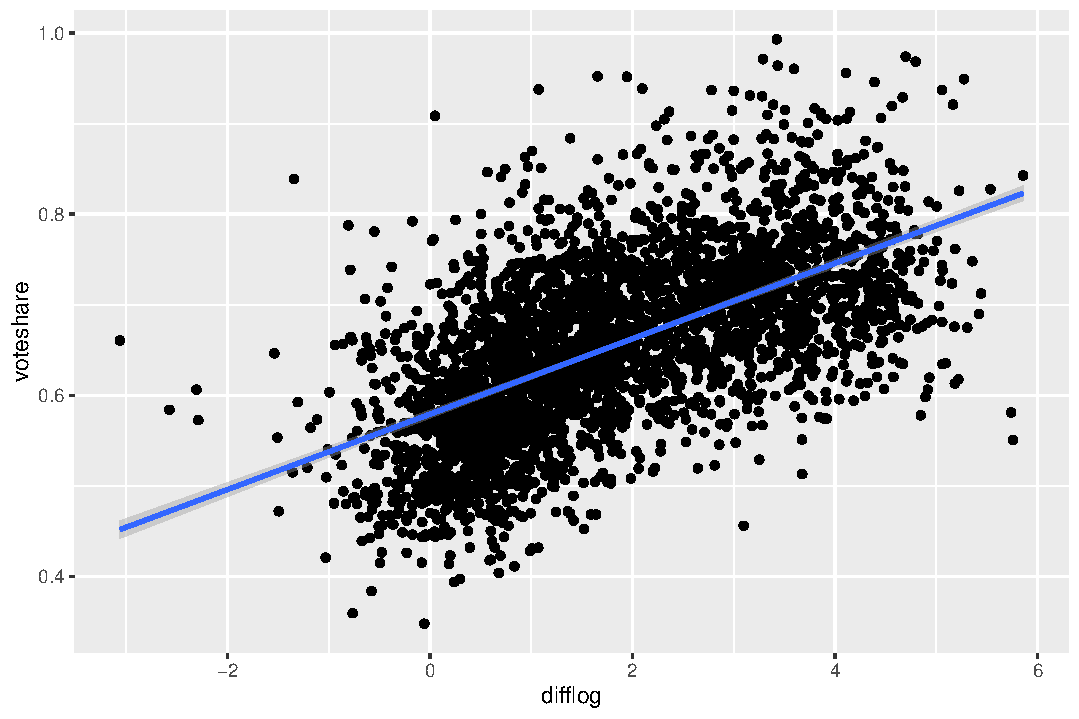
\includegraphics{vdPlot.pdf}
\vspace{.25cm}

\textit{(3)}\\ 
\vspace{.25cm}
\lstinputlisting[language=R, firstline=52, lastline=52]{PS3.R} 
\vspace{.25cm}

\textit{(4)}\\ 
\vspace{.25cm}

\noindent Where $Y$ is \texttt{voteshare} and $x$ is \texttt{difflog} the prediction equation is as follows:

$Y = 0.58 + 0.04x$

\clearpage

\section*{Question 2}

\textit{(1)}\\ 

\vspace{.25cm}

\lstinputlisting[language=R, firstline=61, lastline=62]{PS3.R} 
\begin{table}[!htbp] \centering   \caption{Linear Regression: Presidential Vote Share - Spending Difference}   \label{} \begin{tabular}{@{\extracolsep{5pt}}lc} \\[-1.8ex]\hline \hline \\[-1.8ex]  & \multicolumn{1}{c}{\textit{Dependent variable:}} \\ \cline{2-2} \\[-1.8ex] & presvote \\ \hline \\[-1.8ex]  difflog & 0.024$^{***}$ \\   & (0.001) \\   & \\  Constant & 0.508$^{***}$ \\   & (0.003) \\   & \\ \hline \\[-1.8ex] Observations & 3,193 \\ R$^{2}$ & 0.088 \\ Adjusted R$^{2}$ & 0.088 \\ Residual Std. Error & 0.110 (df = 3191) \\ F Statistic & 307.715$^{***}$ (df = 1; 3191) \\ \hline \hline \\[-1.8ex] \textit{Note:}  & \multicolumn{1}{r}{$^{*}$p$<$0.1; $^{**}$p$<$0.05; $^{***}$p$<$0.01} \\ \end{tabular} \end{table} 

\clearpage

\textit{(2)}\\ 

\vspace{.25cm}

\lstinputlisting[language=R, firstline=65, lastline=68]{PS3.R} 
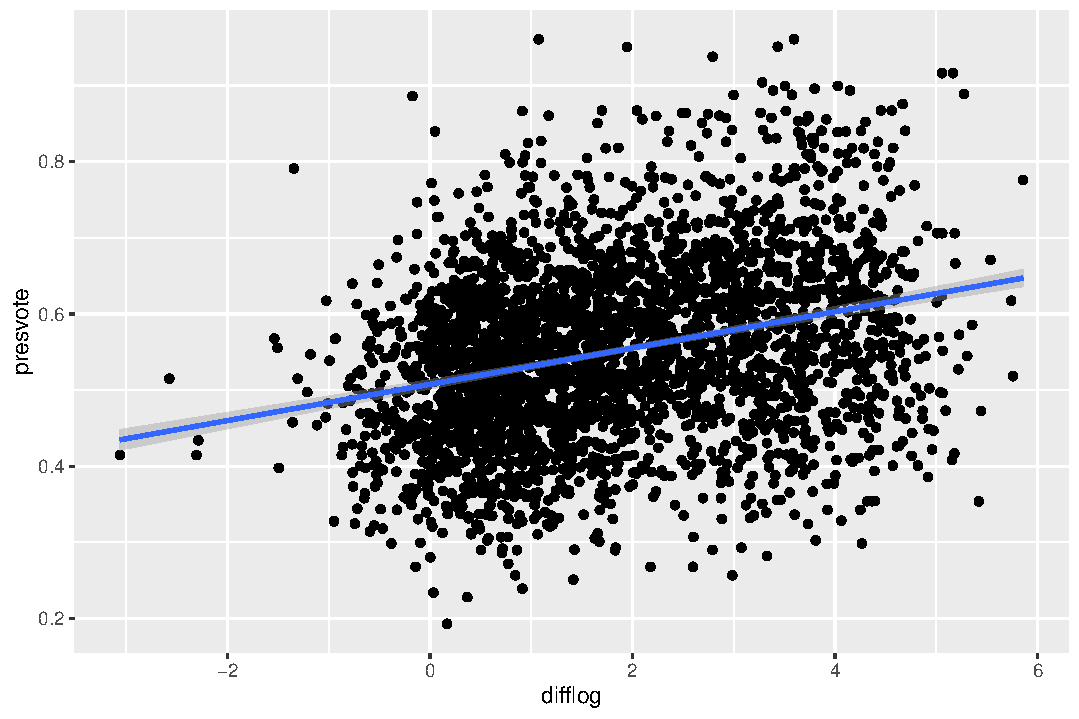
\includegraphics{pdPlot.pdf}
\vspace{.25cm}

\textit{(3)}\\ 
\vspace{.25cm}
\lstinputlisting[language=R, firstline=70, lastline=70]{PS3.R} 
\vspace{.25cm}

\textit{(4)}\\ 
\vspace{.25cm}

\noindent Where $Y$ is \texttt{presvote} and $x$ is \texttt{difflog} the prediction equation is as follows:

$Y = 0.51 + 0.02x$

\clearpage

\section*{Question 3}

\textit{(1)}\\ 

\vspace{.25cm}

\lstinputlisting[language=R, firstline=79, lastline=80]{PS3.R} 
\begin{table}[!htbp] \centering   \caption{Linear Regression: Vote Share - Presidential Vote Share}   \label{} \begin{tabular}{@{\extracolsep{5pt}}lc} \\[-1.8ex]\hline \hline \\[-1.8ex]  & \multicolumn{1}{c}{\textit{Dependent variable:}} \\ \cline{2-2} \\[-1.8ex] & voteshare \\ \hline \\[-1.8ex]  presvote & 0.388$^{***}$ \\   & (0.013) \\   & \\  Constant & 0.441$^{***}$ \\   & (0.008) \\   & \\ \hline \\[-1.8ex] Observations & 3,193 \\ R$^{2}$ & 0.206 \\ Adjusted R$^{2}$ & 0.206 \\ Residual Std. Error & 0.088 (df = 3191) \\ F Statistic & 826.950$^{***}$ (df = 1; 3191) \\ \hline \hline \\[-1.8ex] \textit{Note:}  & \multicolumn{1}{r}{$^{*}$p$<$0.1; $^{**}$p$<$0.05; $^{***}$p$<$0.01} \\ \end{tabular} \end{table} 

\clearpage

\textit{(2)}\\ 

\vspace{.25cm}

\lstinputlisting[language=R, firstline=83, lastline=86]{PS3.R} 
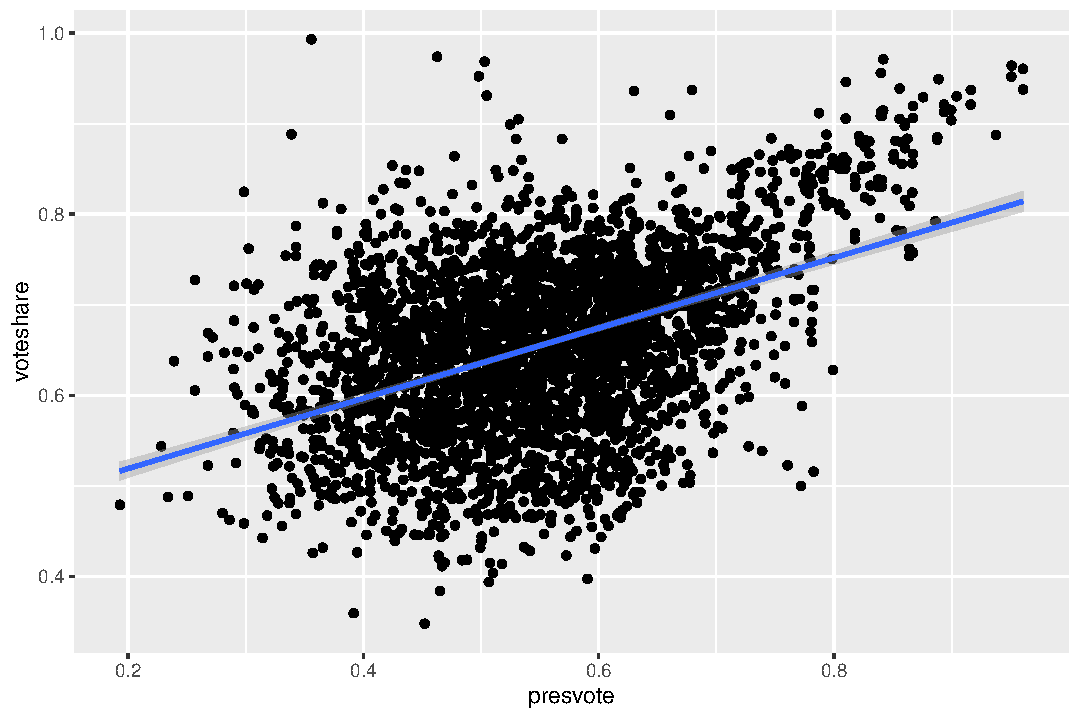
\includegraphics{vpPlot.pdf}
\vspace{.25cm}

\textit{(3)}\\ 
\vspace{.25cm}

\noindent Where $Y$ is \texttt{voteshare} and $x$ is \texttt{presvote} the prediction equation is as follows:

$Y = 0.44 + 0.39x$

\clearpage

\section*{Question 4}

\textit{(1)}\\ 

\vspace{.25cm}

\lstinputlisting[language=R, firstline=94, lastline=95]{PS3.R} 
\begin{table}[!htbp] \centering   \caption{Linear Regression: Residual Model}   \label{} \begin{tabular}{@{\extracolsep{5pt}}lc} \\[-1.8ex]\hline \hline \\[-1.8ex]  & \multicolumn{1}{c}{\textit{Dependent variable:}} \\ \cline{2-2} \\[-1.8ex] & res\_vd \\ \hline \\[-1.8ex]  res\_pd & 0.257$^{***}$ \\   & (0.012) \\   & \\  Constant & $-$0.000 \\   & (0.001) \\   & \\ \hline \\[-1.8ex] Observations & 3,193 \\ R$^{2}$ & 0.130 \\ Adjusted R$^{2}$ & 0.130 \\ Residual Std. Error & 0.073 (df = 3191) \\ F Statistic & 476.975$^{***}$ (df = 1; 3191) \\ \hline \hline \\[-1.8ex] \textit{Note:}  & \multicolumn{1}{r}{$^{*}$p$<$0.1; $^{**}$p$<$0.05; $^{***}$p$<$0.01} \\ \end{tabular} \end{table} 

\clearpage

\textit{(2)}\\ 

\vspace{.25cm}

\lstinputlisting[language=R, firstline=98, lastline=102]{PS3.R} 
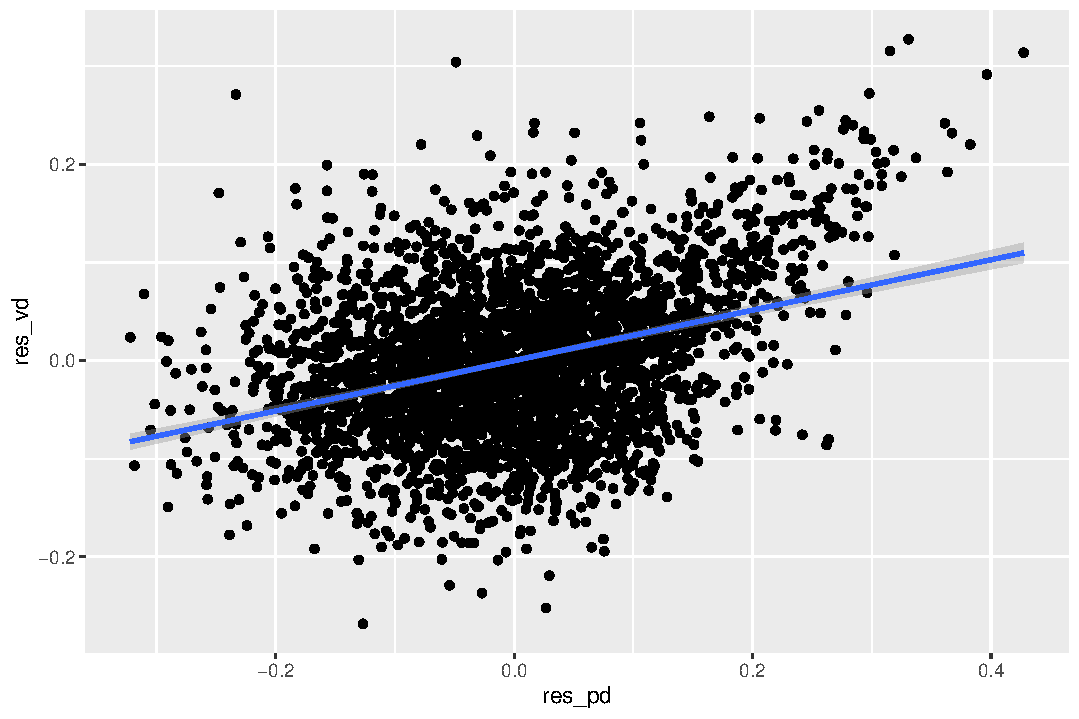
\includegraphics{resPlot.pdf}
\vspace{.25cm}

\textit{(3)}\\ 
\vspace{.25cm}

\noindent Where $Y$ is \texttt{res\_vd} and $x$ is \texttt{res\_pd} the prediction equation is as follows:

$Y = 0.44 + 0.39x$

\clearpage

\section*{Question 5}

\textit{(1)}\\ 

\lstinputlisting[language=R, firstline=109, lastline=110]{PS3.R} 
\begin{table}[!htbp] \centering   \caption{Linear Regression: Vote Share - Spending Difference and Presidential Vote}   \label{} \begin{tabular}{@{\extracolsep{5pt}}lc} \\[-1.8ex]\hline \hline \\[-1.8ex]  & \multicolumn{1}{c}{\textit{Dependent variable:}} \\ \cline{2-2} \\[-1.8ex] & voteshare \\ \hline \\[-1.8ex]  difflog & 0.036$^{***}$ \\   & (0.001) \\   & \\  presvote & 0.257$^{***}$ \\   & (0.012) \\   & \\  Constant & 0.449$^{***}$ \\   & (0.006) \\   & \\ \hline \\[-1.8ex] Observations & 3,193 \\ R$^{2}$ & 0.450 \\ Adjusted R$^{2}$ & 0.449 \\ Residual Std. Error & 0.073 (df = 3190) \\ F Statistic & 1,302.947$^{***}$ (df = 2; 3190) \\ \hline \hline \\[-1.8ex] \textit{Note:}  & \multicolumn{1}{r}{$^{*}$p$<$0.1; $^{**}$p$<$0.05; $^{***}$p$<$0.01} \\ \end{tabular} \end{table} 

\textit{(2)}\\ 

\noindent Where $Y$ is \texttt{voteshare}, $x\textsubscript{1}$ is \texttt{difflog} and $x\textsubscript{2}$ is \texttt{presvote} the prediction equation is as follows:

$Y = 0.45 + 0.04x\textsubscript{1} + 0.26x\textsubscript{2}$
\vspace{.25cm}

\textit{(3)}\\ 

\noindent When using \texttt{R}'s \texttt{summary()} command, we can see the residuals of the two models are the same. The residual model investigated the confounding effects between presvote and difflog's effect on voteshare, so a model including them both as input variables will have the same residuals as the residual model

\end{document}
